% Copyright (c) 2012-2013 by the University of Waikato, Hamilton, NZ. 
% This work is made available under the terms of the 
% Creative Commons Attribution-ShareAlike 3.0 license, 
% http://creativecommons.org/licenses/by-sa/3.0/. 
%
% Version: $Revision$

\chapter{Tools}

\section{Explorer}
ADAMS contains an extended version of the WEKA Explorer. The interface uses
menus instead of buttons to declutter the pre-process tab. Also, it keeps track
of the datasets that the user loads, to make re-loading recent files easier.
This saves a lot of time when working with the same files on a frequent basis.
Furthermore, the user can have an arbitrary number of Explorer sessions in the
same window, distinguished by names. Figure \ref{explorerext} shows the new
interface with the drop-down menu in action.

\begin{figure}[htb]
  \centering
  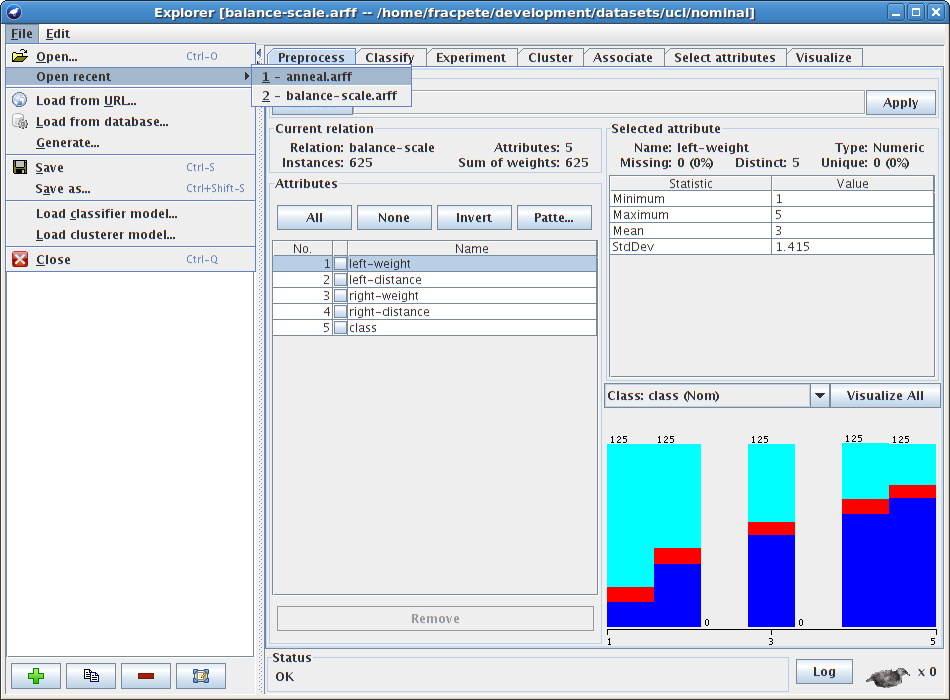
\includegraphics[width=10.0cm]{images/explorerext.png}
  \caption{Explorer interface with menus.}
  \label{explorerext}
\end{figure}

One very useful feature is the notion of \textit{workspaces} in this interface.
You can save the current setup (current dataset, classifiers, clusterers, 
evaluation set up, results, etc.) to a file and restore all of it in one go 
again. Unfortunately, not all data can be stored, such as the log, the undo
history and the built models or visualizations associated with a results.
See Figure \ref{explorerext-workspaces} for the button (highlighted in red) 
that allows you to load/save workspaces.

\begin{figure}[htb]
  \centering
  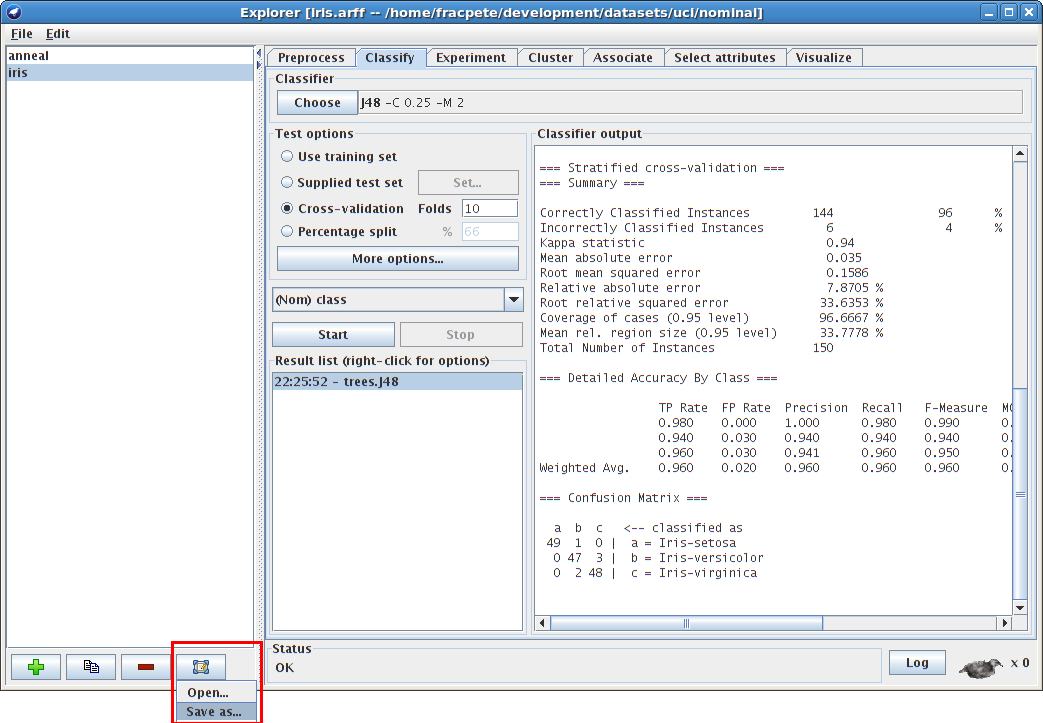
\includegraphics[width=10.0cm]{images/explorerext-workspaces.png}
  \caption{Saving/restoring of workspaces.}
  \label{explorerext-workspaces}
\end{figure}

The extended interface also has a dedicated tab for running experiments, using
the currently loaded dataset and a single classifier. This allows you to 
perform 10 runs of cross-validation instead of the Explorer's default single
run (see Figure \ref{explorerext-experiment}).

\begin{figure}[htb]
  \centering
  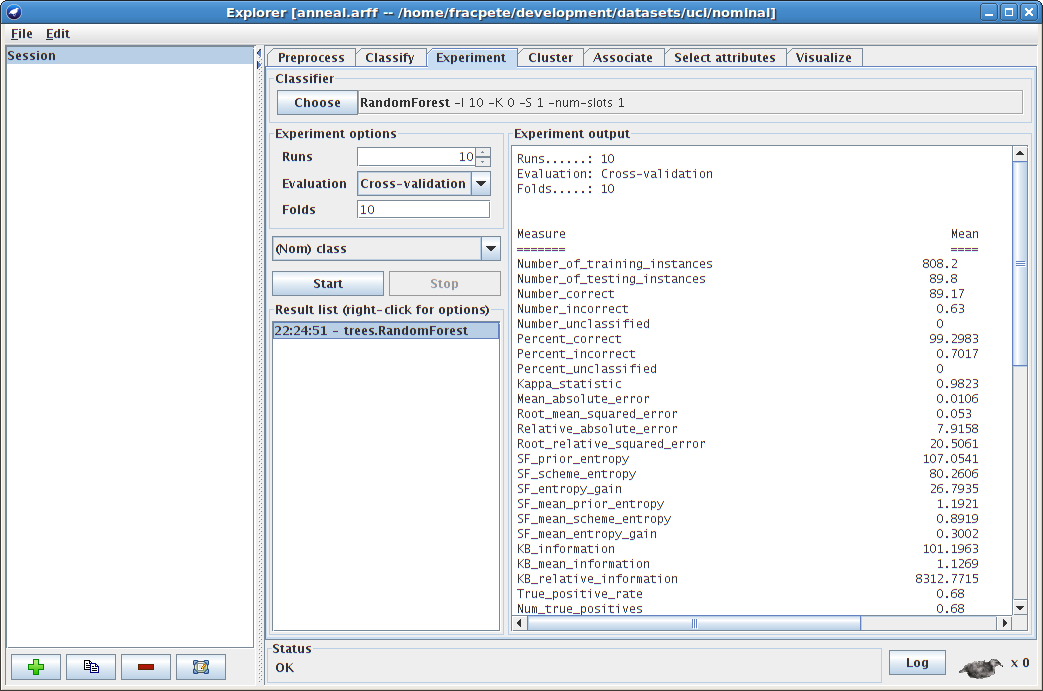
\includegraphics[width=10.0cm]{images/explorerext-experiment.png}
  \caption{Experiment tab in the Explorer.}
  \label{explorerext-experiment}
\end{figure}

\clearpage
\section{Dataset compatibility}

WEKA requires training and test sets to have the same structure, down to the
same name and order of nominal labels. Rather than relying on the error message
in the Explorer, you can use the \textit{Dataset compatibility} tool to 
quickly check whether two or more datasets are actually compatible.

The screenshot in Figure \ref{dataset-compatibility} shows the output when
comparing two datases, one being the original \textit{anneal} UCI dataset
and the other one a transformed version.

\begin{figure}[htb]
  \centering
  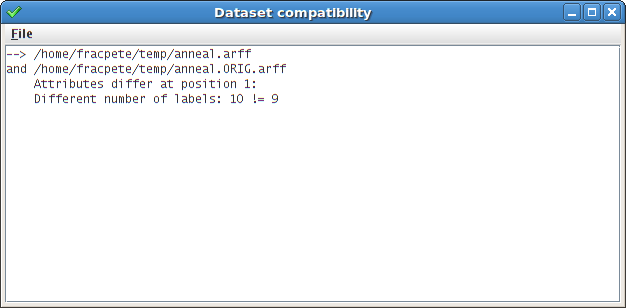
\includegraphics[width=10.0cm]{images/dataset-compatibility.png}
  \caption{Compatibility output for two datasets.}
  \label{dataset-compatibility}
\end{figure}
